%Librerías a usar---------------------------------------------------------------------
\documentclass[11pt, twocolumn]{llncs}
\usepackage[spanish]{babel}
\usepackage[utf8]{inputenc}
\usepackage{multicol}
\usepackage{geometry}
\usepackage{graphicx}
\usepackage{wrapfig}
\usepackage{listings}
\usepackage{hyperref}
\usepackage{tabularx,booktabs,caption}
\newcolumntype{Z}{>{\raggedright}X}
\renewcommand\spanishtablename{Tabla}
\geometry{top=1in, left=1in, right=1in}

%Inicio del documento-----------------------------------------------------------------
\begin{document}
\twocolumn[

%Título y autores---------------------------------------------------------------------
\title{TIEMPO DE EJECUCIÓN DE UN ALGORITMO DE MATRICES CUADRADAS}
\author{
Germán Contreras  \and 
Luciano Grandi  \and
Luis Correa \and 
Rodrigo Aguirre  \\ 
 \email{\{usuario1\}\{usuario2\}\{usuario3\}\{usuario4\} @utem.cl}
}
\institute{Universidad Tecnológica Metropolitana del Estado de Chile, Santiago, Chile
}
\maketitle
\begin{@twocolumnfalse}

%Resumen del documento----------------------------------------------------------------
\begin{abstract}
Breve resumen.

%Palabras Clave-----------------------------------------------------------------------
\textit{Key words:} Datos, paper

\end{abstract}
\end{@twocolumnfalse}
]

%INTRODUCCIÓN------------------------------------------------------------------------
\section{INTRODUCCIÓN}
Las matrices son un tipo de estructura matemática, objeto principal de estudio de la rama del álgebra lineal, relevante en el desarrollo de muchas ciencias. Es utilizada ampliamente para la resolución de sistemas de ecuaciones lineales, derivadas parciales, ecuaciones diferenciales, entre otros; todos estos aplicables a variadas disciplinas como la estadística, economía, física, computación, entre otras.

En las ciencias de la computación, esta estructura es ampliamente utilizada como método de resolución de muchos problemas. Esto se debe a que las matrices son una estructura que agilizan enormemente las operaciones algebraicas, que, utilizando otros métodos, serían tediosos e imprácticos, además de ser una estructura lógica-abstracta fácilmente comprendida por la mente humana, lo que ayuda a la interacción directa con la máquina. Por ejemplo, Las matrices son muy utilizadas en librerías de procesamiento gráfico, debido a su fácil procesamiento vectorial y representación de gráficos tridimensional a bidimensional. 

La informática busca constantemente la optimización de los recursos para la realización de las tareas, principalmente el tiempo y memoria. Debido a que las matrices son una estructura relevante en la mayoría de los procesos informáticos nos es casi imposible no analizar los algoritmos de operación de matrices, sobre todo el de multiplicación, ya que la mayoría de las arquitecturas de procesadores basan sus instrucciones de bajo nivel en sumas y multiplicaciones. 

Utilizando metodologías empíricas, se pretende realizar un experimento de aplicación de un algoritmo de multiplicación de matrices cuadradas, con el fin de analizar el tiempo de ejecución en función del tamaño de datos de entrada n, que en este caso corresponde a la dimensión de las matrices. Con los resultados se espera hallar con el modelo matemático que mejor se ajuste al algoritmo, utilizando técnicas como la regresión lineal. 

Este algoritmo se implementará en lenguaje de programación híbrido C++, reconocido por su alto rendimiento en el manejo de los recursos del sistema. Se aplicará técnicas de programación tradicionales y se utilizará la asignación de memoria dinámica.

Una vez hallado con el modelo matemático se buscará validarlo, realizando un set extra de muestras experimentales que comparen los resultados reales con los obtenidos utilizando el modelo.

A continuación, encontrará una explicación a fondo del propósito, objetivos y metodologías del estudio, así como también el diseño y ejecución del experimento. Usted encontrará un análisis exhaustivo de los resultados obtenidos, así como la conclusión de éste.


%CONTEXTO Y PROPÓSITO DEL EXPERIMENTO------------------------------------------------
\section{CONTEXTO Y PROPÓSITO}\label{contexto_proposito}

Un algoritmo es un conjunto de instrucciones definidas, o secuencias de pasos lógicos que permiten solucionar un problema o realizar una tarea determinada. Estos algoritmos pueden clasificarse acorde a su complejidad, ya sean sencillos o complejos. Al disponer de un algoritmo que funcione correctamente, se nos hace útil determinar ciertos criterios para cuantificar su comportamiento, o en otras palabras, su rendimiento.

Muy seguido se piensa que al hablar de algoritmos sencillos, estos no son competentes. Pero, a la hora de modelar un algoritmo, la sencillez es un componente muy interesante, dado que agiliza el estudio de su eficiencia y su mantenimiento. Cuando hablamos de rendimiento en un algoritmo, este se mide respecto a dos parámetros: el espacio de memoria y el tiempo de ejecución.

Se denomina como tiempo de ejecución de un algoritmo al rango de tiempo t en que un algoritmo comienza su proceso de ejecución hasta el término de este. Este tiempo dependerá de varios factores, tales como la calidad del código o la complejidad del mismo, y los datos de entrada.

Los datos de entrada (dependiendo del tamaño) al interactuar en un algoritmo, tendrán distintos comportamientos y tiempos de ejecución, tal como muchas funciones matemáticas que existen. Esta comparación no es trivial, dado que al saber la complejidad de una función matemática, podemos relacionarla con algún algoritmo y determinar de forma teórica su grado de dificultad. Este grado de dificultad se puede usar para determinar a qué orden de complejidad corresponde cada algoritmo, y así encontrar el que mejor se adapte al problema a solucionar.

Para tal efecto, se desarrollará un algoritmo que pueda crear y multiplicar dos matrices cuadradas de tamaño n. Una matriz es un arreglo bidimensional con un conjunto de datos, ordenados en filas ($i$) y columnas ($j$). Existen diversos tipos de matrices, como las matrices nulas, donde sus datos son solo ceros o las matrices cuadradas como se muestra en la \textit{Fig. 1}, las cuales tienen el mismo número de filas y columnas tal que \textit{n = i = j}.

\begin{figure}
\caption{\textit{\label{fig:matrices}Ejemplo de matrices cuadradas.}}
\centering
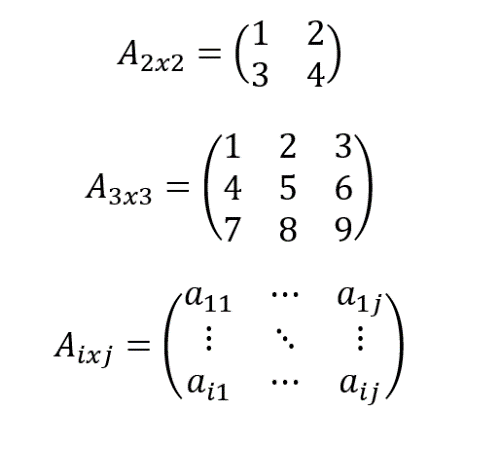
\includegraphics[width=0.3\textwidth]{matrices.png}
\end{figure}

El uso de matrices cuadradas no solo está ligado a la programación o al álgebra clásica, sino que también a la economía en operaciones muy complejas como las descomposiciones de Cholesky y LU. En el ámbito computacional, las matrices son usadas dado su fácil manejo y liviandad para la manipulación de información. Bajo este contexto, son una buena composición para representar diversos tipos de grafos.

La implementación del algoritmo busca formular una función que pueda describir de manera teórica y matemática el comportamiento del tiempo de ejecución en base al tamaño de datos de entrada $n$, por medio de un análisis empírico respecto a la ejecución del algoritmo con distintos valores de entrada de $n$.

Se busca que en base a los valores obtenidos mediante el análisis empírico, estos sean comparados con valores obtenidos en base al modelo matemático formulado, con los mismos valores de entrada $n$ usados anteriormente. Con esto, se espera encontrar un margen de error RDP (\textit{Residual Prediction Deviation}) por cada valor de $n$ usado y explicar los valores RDP que sean interesantes.

El algoritmo en estudio está escrito en lenguaje de programación $C++$. Este algoritmo creará dos matrices cuadradas $A$ y $B$ de tamaño $n$, las cuales estarán pobladas con números enteros positivos aleatorios dentro de un rango definido (desde 1 hasta 100). Con las matrices pobladas, se procederán a multiplicar para formar una nueva matriz cuadrada $C$.

El código del algoritmo es el siguiente:

\lstset{language=, breaklines=true, basicstyle=\footnotesize}
\begin{lstlisting}[frame=single]

#include <iostream>
#include <stdlib.h>
#include <time.h>

using namespace std;

void multmatrix(int n)
{
  int i,j,k;
  long **matriz1=NULL;
  long **matriz2=NULL;
  long **res=NULL;

  matriz1=(long **)malloc(n * sizeof(long *));
  matriz2=(long **)malloc(n * sizeof(long *));
  res=(long **)malloc(n * sizeof(long *));
    
  for (i=0;i<n;i++){
    matriz1[i]=(long *)malloc(n * sizeof(long *));
    matriz2[i]=(long *)malloc(n * sizeof(long *));
    res[i]=(long *)malloc(n * sizeof(long *));
  }
    
  srand(time(NULL));
    
  for(i=0;i<n;i++){
	for(j=0;j<n;j++){
   	  matriz1[i][j]=rand()%100;
      matriz2[i][j]=rand()%100;
    }
  }
  for(i=0;i<n;i++){
    for(j=0;j<n;j++){
      long sum=0;
      for(k=0;k<n;k++){
        sum+=matriz1[j][k]*matriz2[k][i];
      }
      res[j][i]=sum;
    }
  }

  cout<<"Resultado: ";
    for(i=0;i<n;i++){
      for(j=0;j<n;j++){
        cout<<res[i][j];
        cout<<"-";
      }
      cout<<endl;
    }
  }
}

int main(){
  int n;
  cout<<"Valor n: ";
  cin>>n;
  getchar();
  unsigned t0, t1;
  t0=clock();
  multmatrix(n);
  t1=clock();
  double time=(double(t1-t0)/CLOCKS_PER_SEC);
  cout<<"TIEMPO DE EJECUCION: "<<time;
  return 0;
}

\end{lstlisting}

El código diseñado está modelado para recibir valores de entrada de $n$ en un rango aproximado entre 1 a 10000. Para tal efecto, las matrices declaradas tendrán asignación de memoria. Y además, se usa la librería time.h para poder calcular los tiempos de ejecución del algoritmo.

%OBJETIVOS---------------------------------------------------------------------------
\section{OBJETIVOS DEL EXPERIMENTO}\label{objetivos}
Los objetivos son las razones por las cuales se lleva a cabo una acción a corto, mediano o largo plazo. La importancia de los objetivos reside en el hecho de permitir el orden de forma eficiente para saber cómo trabajar o actuar y qué cosas o resultados buscar.

\subsection{Objetivo general}
Medir el tiempo de ejecución de un algoritmo de multiplicación de matrices cuadradas con datos de valores de entrada $n$ y realizar un análisis empírico de los resultados.

\subsection{Objetivos específicos}
\begin{itemize}
    \item Diseñar y ejecutar un experimento a base de un algoritmo.
    \item Recopilar muestras de datos experimentales de la aplicación del algoritmo.
    \item Analizar los resultados obtenidos en el experimento.
    \item Graficar los resultados obtenidos.
    \item Determinar el modelo matemático en función al tiempo que se ajusta al problema.
    \item Validar el modelo matemático obtenido ejecutando nuevamente el experimento con una serie de datos distintos a los usados anteriormente.
    \item Comparar los resultados empíricos con los predichos en el modelo obtenido.
    \item Comentar los valores RDP y explicar el porcentaje obtenido.
\end{itemize}

%METODOLOGÍA-------------------------------------------------------------
\section{METODOLOGÍA}\label{metodología}
Una buena forma de conseguir resultados esperados, es implementar una metodología que se adapte a las necesidades del estudio, así generando una visión clara y concisa de las acciones relevantes consideradas en la realización del experimento.

\subsection{Reuniones y roles de trabajo}
Para el desarrollo de la actividad, se determinaron sesiones de estudio con una duración de al menos dos horas cada tres días. En cada sesión, se distribuyeron las tareas para cada integrante del equipo, además de planificar las sesiones siguientes.

\subsection{Etapas del experimento}
Para la elaboración del experimento, se eligió un lenguaje de programación fácil de dominar para los integrantes del grupo. Entre las alternativas propuestas por cada integrante (Java, Python, Ruby, C++), se determinó el uso de $C++$ para el desarrollo del algoritmo.

Con el lenguaje elegido, se comenzó a diseñar el algoritmo para multiplicar dos matrices. Cada integrante diseñó un algoritmo respectivo, así escogiendo el más adecuado y eficiente, testeando diversos valores de entrada de $n$ para su correcto funcionamiento.

El diseño del algoritmo se basa en la implementación de dos matrices creadas de forma dinámica dependiendo del valor de entrada de $n$ mediante consola. Para la operación de multiplicación se debe considerar que teniendo dos matrices $A$ y $B$, estas son multiplicables si el número de columnas $i$ de la matriz $A$ es igual que el número de filas $j$ de la matriz $B$. Para la obtención de la matriz producto $C$ se usó la siguiente ecuación matemática:

\begin{equation}
A_{ij} \times B_{jk} = C_{ik}
\end{equation}

En la \textit{Eq. (1)}, el valor del elemento $C_{ik}$ de la matriz producto se obtiene multiplicando cada elemento de la fila $i$ de la matriz $A$ por cada elemento de la columna $j$ de la matriz $B$ y sumándolos. En la \textit{Fig. 2} se muestra el procedimiento de multiplicación de dos matrices pobladas.

\begin{figure}
\caption{\textit{\label{fig:multiplicacion}Proceso de multiplicación de dos matrices.}}
\centering
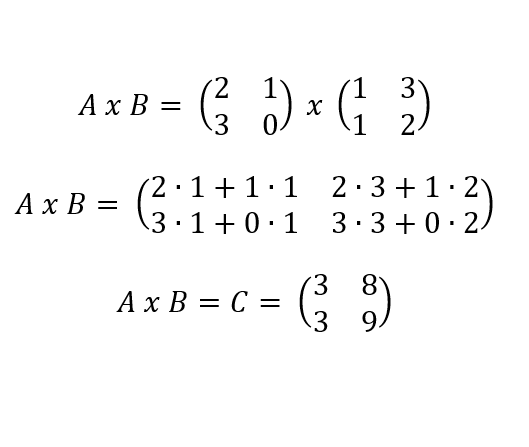
\includegraphics[width=0.4\textwidth]{multiplicacion.png}
\end{figure}

Además, se implementó en el código la librería \textit{time.h} para la medición del tiempo de ejecución de la creación de las matrices. Con la librería implementada, se procedió a utilizar la función \textit{clock()}, la cual calcula el tiempo en segundos en el momento que es llamada. A continuación se muestra el código para el cálculo del tiempo de ejecución:

\lstset{language=, breaklines=true, basicstyle=\footnotesize}
\begin{lstlisting}[frame=single]

//Funcion multiplicacion de matrices
void multmatrix(int n){
...
}

//Funcion principal
int main(){
  ...
  //Creacion de variables enteras sin signo
  unsigned t0, t1;
  
  //Llamada de la funcion clock() para el comienzo del tiempo del algoritmo
  t0=clock();
  
  //Llamada de la funcion multiplicacion de matrices
  multmatrix(n);
  
  //Llamada de la funcion clock() para el termino del tiempo del algoritmo
  t1=clock();
  
  //Creacion de variable con el tiempo final de ejecucion del algoritmo
  double time=(double(t1-t0)/CLOCKS_PER_SEC);
  ...
}

\end{lstlisting}

Todo el código implementado para la elaboración del experimento está en la sección 2 de este documento (CONTEXTO Y PROPÓSITO).

Cada tiempo de ejecución entregado por el código fue recolectado y tabulado, con el fin de generar un gráfico en las coordenadas $x$ e $y$ en el plano cartesiano obteniendo su regresión adecuada y respectiva formulación del modelo matemático.

\subsection{Herramientas de hardware}
Se ha usado para el experimento un Notebook con las siguientes características:

\begin{itemize}
    \item $CPU$: AMD Ryzen 3 2200U con Radeon Vega Mobile 2,5GHz quadcore.
    \item $RAM$: 8 GB (1 x 8 GB) DDR4 a 2400mhz SODIMM.
    \item $Memoria$: SSD NVME Western Digital de 250 GB.
    \item \textit{Sistemas Operativos}: Windows 10 Pro x64 y Manjaro x64 Kernell Linux 5.9.10-1.
\end{itemize}

Se ha propuesto el uso de dos sistemas operativos para la comparación de los tiempos de ejecución de $n$ en cada sistema en particular.

\subsection{Herramientas de software}
Para el desarrollo del experimento se ha usado el lenguaje de programación $C++$, junto con el entorno de desarrollo \textit{Code::Blocks V22.04 x64} y con el compilador \textit{ggc compiler} integrado. Para la tabulación y regresión del modelo matemático se ha usado el programa \textit{Microsoft Excel}. Para el diseño de gráficos de funciones se ha utilizado $Geogebra$, un software matemático online.

%DISEÑO DEL EXPERIMENTO-------------------------------------------------------------
\section{DISEÑO DEL EXPERIMENTO}\label{diseño}


%EJECUCIÓN DEL EXPERIMENTO-------------------------------------------------------------
\section{EJECUCIÓN DEL EXPERIMENTO}\label{ejecucion}
El tiempo que tomó realizar este experimento
fue de aproximadamente una hora y media,
ya que se tomaron un total de 78 mediciones
para 13 valores de n. Esto debido a que se realizaron las pruebas en distintos sistemas operativos dentro de la misma máquina.

No se presentaron problemas en la ejecución del experimento, pero si una diferencia notable en la ejecución del algoritmo.

%RESULTADOS OBTENIDOS-------------------------------------------------------------
\section{RESULTADOS OBTENIDOS}\label{resultados}


%------------------------------------------------------------------------

\end{document}